\documentclass[12pt,a4paper]{article}

% ============================================================================
% PACKAGES
% ============================================================================
\usepackage[utf8]{inputenc}
\usepackage[T1]{fontenc}
\usepackage[margin=1in]{geometry}
\usepackage{graphicx}
\usepackage{amsmath}
\usepackage{amssymb}
\usepackage{booktabs}
\usepackage{listings}
\usepackage{xcolor}
\usepackage{tikz}
\usepackage{float}
\usepackage{caption}
\usepackage{array}
\usepackage{cite}
\usepackage{setspace}
\usepackage[hidelinks,
    pdftitle={Battery Monitoring System Using ESP32 and C Firmware},
    pdfauthor={Pradumon Sahani}
]{hyperref}

\usetikzlibrary{shapes.geometric, arrows.meta, positioning, fit, backgrounds, calc}

% ============================================================================
% TYPOGRAPHY & LISTINGS CONFIGURATION
% ============================================================================
\onehalfspacing
\captionsetup{font=small, labelfont=bf}

\definecolor{codebg}{RGB}{248, 248, 248}
\definecolor{codecomment}{RGB}{0, 110, 0}
\definecolor{codekeyword}{RGB}{0, 0, 180}
\definecolor{codestring}{RGB}{163, 21, 21}
\definecolor{codenum}{RGB}{120, 120, 120}

\lstdefinestyle{CStyle}{
    language=C,
    backgroundcolor=\color{codebg},
    commentstyle=\color{codecomment}\itshape,
    keywordstyle=\color{codekeyword}\bfseries,
    numberstyle=\tiny\color{codenum},
    stringstyle=\color{codestring},
    basicstyle=\ttfamily\scriptsize,
    breakatwhitespace=false,
    breaklines=true,
    captionpos=b,
    keepspaces=true,
    numbers=left,
    numbersep=7pt,
    showspaces=false,
    showstringspaces=false,
    showtabs=false,
    tabsize=4,
    frame=single,
    rulecolor=\color{black!30},
    columns=flexible
}
\lstset{style=CStyle}

% ============================================================================
% DOCUMENT START
% ============================================================================
\begin{document}

% ----------------------------------------------------------------------------
% 1. TITLE PAGE
% ----------------------------------------------------------------------------
\begin{titlepage}
    \centering
    \vspace*{0.8cm}

    {\Large \textbf{INDIAN INSTITUTE OF TECHNOLOGY MADRAS}\par}
    \vspace{0.3cm}
    {\large BS Electronics Engineering\par}
    \vspace{1.2cm}

    \rule{\linewidth}{0.5mm}\\[0.5cm]
    {\LARGE \bfseries Battery Monitoring System Using ESP32 and C Firmware\par}
    \vspace{0.4cm}
    \rule{\linewidth}{0.5mm}\\[1.0cm]

    {\large Electronics Project Proposal and Technical Design Report\par}
    \vspace{1.6cm}

    \begin{tabular}{rl}
        \textbf{Submitted by:} & Pradumon Sahani \\
        \textbf{Program:} & BS Electronics Engineering \\
        \textbf{Institution:} & Indian Institute of Technology Madras (IIT Madras) \\
        \textbf{Roll no.:} & 26T3Q1S2ESQ1S200903 \\
    \end{tabular}

    \vfill

    {\large November 2026\par}
\end{titlepage}

\pagenumbering{roman}

% ----------------------------------------------------------------------------
% 2. ABSTRACT & 3. KEYWORDS
% ----------------------------------------------------------------------------
\begin{abstract}
Lithium-ion (Li-ion) rechargeable batteries are central to modern portable electronics, Internet of Things (IoT) devices, and embedded instrumentation owing to their high energy density and low self-discharge. However, operating a single-cell Li-ion battery outside its safe voltage and thermal envelope leads to rapid capacity degradation and potential thermal safety hazards. In this project proposal, I present the complete hardware and firmware design of an embedded Battery Monitoring System (BMS) built around the ESP32 DevKit V1 microcontroller and programmed in C using the Espressif IoT Development Framework (ESP-IDF). The proposed system monitors a single-cell 3.7~V nominal (4.2~V fully charged) Li-ion battery by stepping down its terminal voltage through a $100\text{ k}\Omega / 100\text{ k}\Omega$ resistive voltage divider (buffered with a $100\text{ nF}$ bypass capacitor) into the ESP32 12-bit Successive Approximation Register (SAR) Analog-to-Digital Converter (ADC). State of Charge (SOC) is estimated using an 11-point resting Open-Circuit Voltage (OCV) lookup table with piecewise linear interpolation. Cell surface temperature is acquired via a DS18B20 1-Wire digital thermometer with CRC-8 verification, threshold-based hysteresis logic generates low-battery and high-temperature warnings, and real-time telemetry is rendered on an SSD1306 $128 \times 64$ OLED display over I2C. Because this document is submitted as a project idea and complete design specification prior to physical laboratory assembly, all theoretical calculations, complete ESP-IDF C firmware architecture, expected operational behavior, and planned bench validation protocols are explicitly distinguished from future empirical hardware measurements.
\end{abstract}

\vspace{0.35cm}
\noindent\textbf{Keywords:} Battery Monitoring System, ESP32, ESP-IDF, C Firmware, Li-ion Battery, SAR ADC, Voltage Divider, State of Charge (SOC), Linear Interpolation, DS18B20, 1-Wire Protocol, SSD1306 OLED, I2C, FreeRTOS.

\newpage
\tableofcontents
\newpage
\listoffigures
\listoftables
\newpage

\pagenumbering{arabic}

% ----------------------------------------------------------------------------
% 4. INTRODUCTION
% ----------------------------------------------------------------------------
\section{Introduction}
\label{sec:introduction}

Rechargeable lithium-ion (Li-ion) cells have become the standard power source across portable consumer products, wireless sensor nodes, medical wearables, and student embedded prototypes due to their high gravimetric energy density, negligible memory effect, and high nominal cell voltage (3.6~V--3.7~V) compared with nickel-based chemistries~\cite{reddy_linden}. Despite these advantages, Li-ion chemistry requires strict electrical and thermal supervision. Discharging a single cell below its cutoff threshold (typically 2.8~V--3.0~V) causes copper dissolution from the anode current collector and irreversible capacity loss, while elevated temperatures accelerate solid-electrolyte interphase (SEI) growth, electrolyte decomposition, and thermal runaway risk~\cite{plett_bms1}.

Commercial electric vehicle battery packs utilize complex multi-cell Battery Management Systems (BMS) featuring isolated cell-monitoring ASICs, active balancing, and Kalman-filter-based estimation~\cite{plett_bms2}. In contrast, standalone single-cell embedded systems benefit from a compact, low-cost, microcontroller-driven monitoring unit that provides immediate voltage, charge percentage, temperature, and fault-warning feedback without prohibitive hardware overhead.

As my individual project idea for BS Electronics Engineering at IIT Madras, I propose an embedded Battery Monitoring System centered on the ESP32 DevKit V1 platform programmed in C under the ESP-IDF framework~\cite{espressif_espidf}. The proposed design integrates a resistive voltage divider for safe ADC interfacing, a DS18B20 1-Wire digital temperature sensor~\cite{analog_ds18b20}, and an SSD1306 $128 \times 64$ monochrome OLED display over I2C~\cite{solomon_ssd1306}. This report documents the complete theoretical foundation, circuit schematic, mathematical formulation, modular ESP-IDF C firmware design, and structured validation plan intended for subsequent prototype implementation.

% ----------------------------------------------------------------------------
% 5. PROBLEM STATEMENT
% ----------------------------------------------------------------------------
\section{Problem Statement}
\label{sec:problem_statement}

Small-scale embedded electronics powered by single-cell 3.7~V Li-ion batteries frequently lack integrated state-of-charge and thermal monitoring. Designing a reliable microcontroller-based monitoring unit presents four specific engineering challenges:

\begin{enumerate}
    \item \textbf{Voltage Level Incompatibility:} A fully charged single-cell Li-ion battery reaches 4.20~V, which exceeds the 3.3~V maximum operating voltage of the ESP32 GPIO and ADC pins~\cite{espressif_esp32_ds}. Direct connection risks permanent damage to the microcontroller.
    \item \textbf{ADC Non-Linearity and Reference Variation:} The ESP32 internal 12-bit SAR ADC exhibits chip-to-chip reference voltage variation and quantization noise, requiring resistive scaling into the linear region, factory eFuse calibration, and multi-sample averaging.
    \item \textbf{Non-Linear Voltage-to-Charge Mapping:} A Li-ion battery does not discharge linearly with voltage; it exhibits a flat mid-discharge plateau between roughly 3.60~V and 3.90~V. Simple linear scaling between 3.0~V and 4.2~V produces substantial percentage error.
    \item \textbf{Thermal Safety Blindness:} Without continuous cell-surface temperature sensing and hysteresis-controlled warnings, abnormal heating during heavy discharge or fault conditions can go undetected.
\end{enumerate}

% ----------------------------------------------------------------------------
% 6. OBJECTIVES
% ----------------------------------------------------------------------------
\section{Objectives}
\label{sec:objectives}

The specific technical objectives of this proposed project are:

\begin{enumerate}
    \item To design a low-drain resistive voltage divider ($R_1 = R_2 = 100\text{ k}\Omega$ with a $100\text{ nF}$ filter capacitor) that safely scales a 3.0~V--4.2~V Li-ion cell into the calibrated operating window of ESP32 ADC1.
    \item To design complete, modular ESP-IDF v5.x C firmware that initializes the SAR ADC, applies line-fitting eFuse calibration, averages 64 consecutive samples, and reconstructs terminal battery voltage.
    \item To implement an 11-point OCV-to-SOC lookup table with piecewise linear interpolation and boundary clamping to estimate battery percentage.
    \item To interface a DS18B20 digital temperature sensor via the 1-Wire protocol with 8-bit CRC verification to track battery temperature at $0.0625\,^\circ\text{C}$ resolution.
    \item To implement hysteresis-based low-battery ($\le 3.30\text{ V}$ or $\le 15\%$) and high-temperature ($\ge 45.0\,^\circ\text{C}$) warning logic.
    \item To drive an SSD1306 $128 \times 64$ OLED screen over the ESP32 I2C master bus to display real-time voltage, SOC percentage, temperature, and active alerts.
    \item To establish a quantitative theoretical error analysis and benchtop verification plan for hardware validation.
\end{enumerate}

% ----------------------------------------------------------------------------
% 7. BACKGROUND AND RELATED CONCEPTS
% ----------------------------------------------------------------------------
\section{Background and Related Concepts}
\label{sec:background}

\subsection{ESP32 Microcontroller Architecture}
The ESP32 DevKit V1 houses the ESP32-WROOM-32 module, built around a dual-core 32-bit Xtensa LX6 microprocessor operating at up to 240~MHz~\cite{espressif_esp32_ds, espressif_esp32_trm}. It integrates 520~KB of on-chip SRAM, 448~KB of ROM, 4~MB of external SPI flash, integrated 2.4~GHz Wi-Fi and Bluetooth radios, two 12-bit SAR ADCs, two hardware I2C controllers, SPI, UART, and multiplexed GPIO pins. The core operates at 3.3~V (3.0~V--3.6~V range), supplied on the DevKit V1 by an onboard 5~V-to-3.3~V low-dropout (LDO) linear regulator fed from USB.

\subsection{ESP32 SAR ADC Operation and Calibration}
The ESP32 provides two 12-bit SAR ADCs: ADC1 (8 channels on GPIO32--GPIO39) and ADC2 (10 channels)~\cite{espressif_esp32_trm}. For this design, ADC1 Channel~6 (GPIO34) is selected for two reasons: (a) GPIO34 is an input-only pin, preserving bidirectional GPIOs for digital buses, and (b) ADC1 remains completely independent of the Wi-Fi radio, whereas ADC2 cannot operate concurrently with Wi-Fi.

A 12-bit SAR ADC quantizes analog inputs into codes $D \in [0, 4095]$. The ESP32 internal reference voltage is nominally $V_{\text{ref}} \approx 1100\text{ mV}$ but varies across individual chips between roughly 1000~mV and 1200~mV due to manufacturing tolerances. Configurable input attenuation (0~dB, 2.5~dB, 6~dB, and 12~dB—previously labelled 11~dB in earlier ESP-IDF releases) extends the measurable input span~\cite{espressif_espidf}. At 12~dB attenuation, the ESP32 can measure voltages up to approximately 2.5~V--3.1~V depending on silicon revision, with best linearity between approximately 150~mV and 2450~mV. ESP-IDF provides a Line-Fitting calibration scheme backed by factory-programmed eFuse data to map raw ADC codes directly to calibrated millivolts.

\subsection{Voltage Divider Principle}
A passive two-resistor voltage divider attenuates $V_{\text{battery}}$ to a safe fraction $V_{\text{adc}}$. Resistor selection balances continuous battery drain against source impedance seen by the ADC sample-and-hold capacitor. Selecting $R_1 = R_2 = 100\text{ k}\Omega$ restricts battery drain to $21\,\mu\text{A}$ at 4.2~V while presenting a DC Thevenin resistance of $50\text{ k}\Omega$. Placing a $100\text{ nF}$ ceramic bypass capacitor ($C_f$) across $R_2$ supplies instantaneous charge to the internal SAR sampling capacitor during acquisition and creates a low-pass filter with cutoff frequency $f_c = 1 / (2\pi R_{\text{th}} C_f) \approx 31.8\text{ Hz}$, attenuating high-frequency switching noise.

\subsection{Li-ion Voltage Characteristics and SOC Estimation}
A standard 3.7~V nominal Li-ion cell (such as an 18650 NMC/LCO cell) operates from 4.20~V (100\% SOC) down to 3.00~V (0\% SOC)~\cite{reddy_linden}. The discharge profile falls steeply from 4.20~V to 3.90~V, flattens considerably across 3.90~V--3.55~V, and drops sharply below 3.50~V. Common SOC estimation methods include~\cite{plett_bms2}:
\begin{itemize}
    \item \textbf{Voltage-Based Lookup and Interpolation:} Uses resting terminal voltage mapped through an empirical OCV--SOC curve. It requires no current-shunt circuitry and minimal CPU cycles, though it is affected by load current sag and temperature.
    \item \textbf{Coulomb Counting:} Integrates measured current over time. It tracks dynamic loads accurately over short intervals but accumulates sensor offset drift without periodic OCV recalibration.
    \item \textbf{Kalman Filtering:} Fuses an equivalent-circuit electrochemical model with voltage, current, and temperature measurements for high accuracy at significantly higher hardware and algorithmic complexity.
\end{itemize}
Because this project targets a low-cost, minimal-component single-cell monitor, piecewise linear OCV interpolation is selected as the primary estimation method.

\subsection{DS18B20 1-Wire Temperature Measurement}
The DS18B20 is a digital temperature sensor communicating over a single open-drain 1-Wire data bus (DQ) pulled up to 3.3~V through a $4.7\text{ k}\Omega$ resistor~\cite{analog_ds18b20}. It operates from $-55\,^\circ\text{C}$ to $+125\,^\circ\text{C}$ with $\pm 0.5\,^\circ\text{C}$ accuracy between $-10\,^\circ\text{C}$ and $+85\,^\circ\text{C}$. At its default 12-bit resolution ($0.0625\,^\circ\text{C}$/LSB), conversion requires up to 750~ms, and the 9-byte scratchpad includes an 8-bit CRC byte to detect bus transmission errors.

\subsection{I2C Communication and SSD1306 OLED Display}
The Inter-Integrated Circuit (I2C) bus uses two open-drain lines—Serial Data (SDA) and Serial Clock (SCL)—operating at 100~kHz (Standard-mode) or 400~kHz (Fast-mode)~\cite{nxp_i2c}. The SSD1306 controller drives a $128 \times 64$ monochrome OLED panel using an internal 1024-byte Graphic Display Data RAM (GDDRAM) organized into 8 pages of 128 columns~\cite{solomon_ssd1306}. Standard 0.96-inch I2C OLED modules use 7-bit address \texttt{0x3C}, operate directly at 3.3~V logic, and offer high readability without a backlight.

\subsection{FreeRTOS, ESP-IDF, and Modular C Programming}
ESP-IDF is Espressif's official CMake-based C/C++ SDK built atop an SMP FreeRTOS kernel~\cite{espressif_espidf, barry_freertos}. Firmware starts in \texttt{app\_main()}, which executes as a FreeRTOS task. Periodic execution uses non-blocking \texttt{vTaskDelay()}, freeing the scheduler during idle intervals. Structuring the C firmware with fixed-width integer types (\texttt{<stdint.h>}), \texttt{struct} state records (\texttt{bms\_data\_t}, \texttt{soc\_point\_t}), dedicated single-responsibility functions, and explicit \texttt{esp\_err\_t} error propagation follows rigorous embedded C engineering practice~\cite{kr_c}.

% ----------------------------------------------------------------------------
% 8. HARDWARE COMPONENTS AND SPECIFICATIONS
% ----------------------------------------------------------------------------
\section{Hardware Components and Specifications}
\label{sec:hardware_specs}

Table~\ref{tab:hw_specs} lists all selected hardware components and their technical parameters for the proposed system.

\begin{table}[H]
\centering
\caption{Selected Hardware Components and Technical Specifications}
\label{tab:hw_specs}
\renewcommand{\arraystretch}{1.22}
\begin{tabular}{@{}p{3.2cm}p{3.6cm}p{7.8cm}@{}}
\toprule
\textbf{Component} & \textbf{Model / Value} & \textbf{Key Electrical \& Functional Specifications} \\
\midrule
Microcontroller & ESP32 DevKit V1 (ESP32-WROOM-32) & Dual-core Xtensa LX6 up to 240~MHz; 520~KB SRAM; 4~MB flash; 3.3~V logic; 12-bit SAR ADC (ADC1/ADC2); hardware I2C and UART~\cite{espressif_esp32_ds}. \\
Li-ion Battery & Single-cell 18650 Li-ion & Nominal voltage: 3.7~V; fully charged: 4.20~V; cutoff: 3.00~V; typical capacity: 2200--2600~mAh~\cite{reddy_linden}. \\
Voltage Divider Resistors & $R_1 = 100\text{ k}\Omega$, $R_2 = 100\text{ k}\Omega$ (1\% Metal Film) & Division ratio 0.5; scales 4.20~V to 2.10~V; quiescent drain $21\,\mu\text{A}$ at 4.20~V. \\
ADC Filter Capacitor & $C_f = 100\text{ nF}$ (Ceramic X7R) & Connected across $R_2$; stabilizes SAR sampling capacitor and forms a 31.8~Hz low-pass filter. \\
Temperature Sensor & DS18B20 (TO-92 or Waterproof Probe) & 1-Wire digital sensor; $-55\,^\circ\text{C}$ to $+125\,^\circ\text{C}$; $\pm 0.5\,^\circ\text{C}$ accuracy ($-10\,^\circ\text{C}$ to $+85\,^\circ\text{C}$); 12-bit default ($0.0625\,^\circ\text{C}$)~\cite{analog_ds18b20}. \\
1-Wire Pull-Up Resistor & $R_{\text{pu}} = 4.7\text{ k}\Omega$ (5\% Carbon/Metal Film) & Connects DS18B20 DQ line to 3.3~V rail per datasheet specification~\cite{analog_ds18b20}. \\
OLED Display & SSD1306 $128 \times 64$ (0.96-inch I2C) & Monochrome self-emissive OLED; 3.3~V supply; I2C address \texttt{0x3C}; 400~kHz Fast-mode capable~\cite{solomon_ssd1306}. \\
\bottomrule
\end{tabular}
\end{table}

% ----------------------------------------------------------------------------
% 9. SYSTEM ARCHITECTURE
% ----------------------------------------------------------------------------
\section{System Architecture}
\label{sec:system_architecture}

The proposed system follows a modular four-stage architecture: sensing, analog signal conditioning, embedded digital processing on the ESP32, and local human-machine visualization. Figure~\ref{fig:system_block} presents the complete system block diagram.

\begin{figure}[H]
\centering
\resizebox{\linewidth}{!}{%
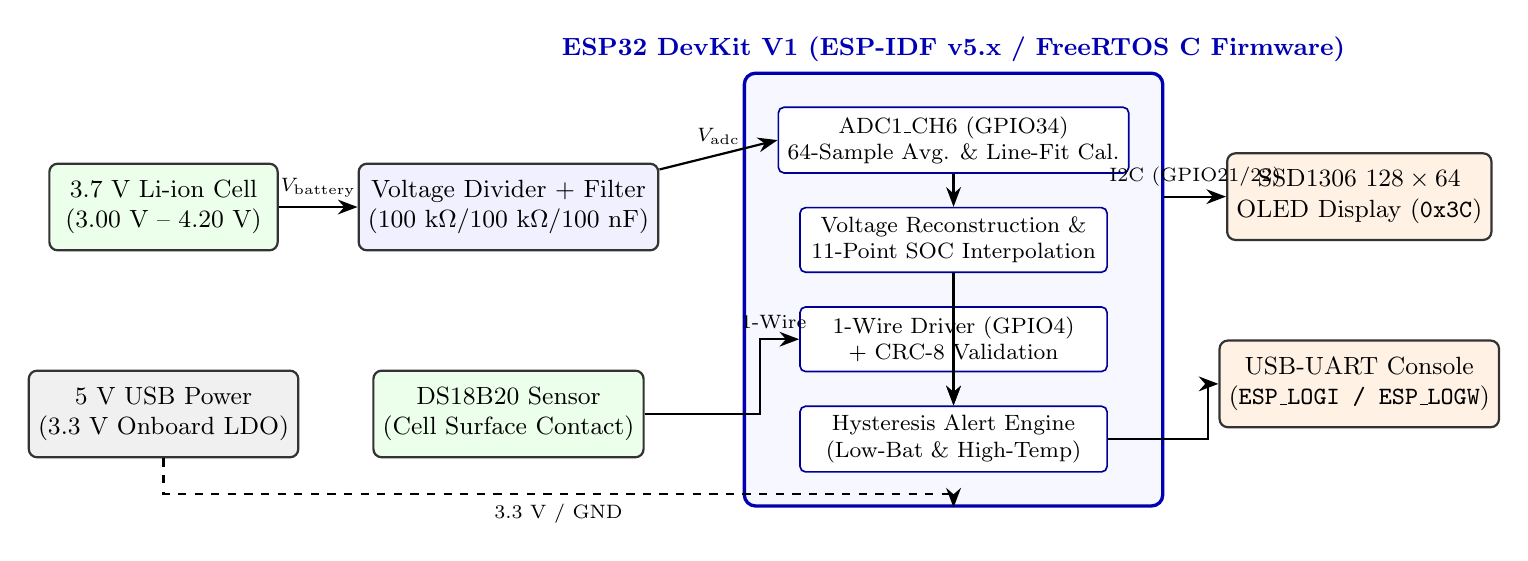
\begin{tikzpicture}[
    node distance=1.0cm and 1.2cm,
    block/.style={rectangle, draw=black!80, thick, rounded corners=3pt, minimum width=2.9cm, minimum height=1.1cm, align=center, font=\small, fill=blue!6},
    sensor/.style={rectangle, draw=black!80, thick, rounded corners=3pt, minimum width=2.9cm, minimum height=1.1cm, align=center, font=\small, fill=green!8},
    output/.style={rectangle, draw=black!80, thick, rounded corners=3pt, minimum width=3.0cm, minimum height=1.1cm, align=center, font=\small, fill=orange!10},
    mcu/.style={rectangle, draw=blue!70!black, very thick, rounded corners=4pt, fill=blue!3, inner sep=12pt},
    proc/.style={rectangle, draw=blue!60!black, semithick, rounded corners=2pt, minimum width=3.9cm, minimum height=0.82cm, align=center, font=\footnotesize, fill=white},
    arr/.style={-{Stealth[length=2.5mm]}, thick}
]

\node[sensor] (bat) {3.7 V Li-ion Cell\\(3.00 V -- 4.20 V)};
\node[block, right=1.0cm of bat] (vdiv) {Voltage Divider + Filter\\($100\text{ k}\Omega / 100\text{ k}\Omega / 100\text{ nF}$)};
\node[sensor, below=1.5cm of vdiv] (temp) {DS18B20 Sensor\\(Cell Surface Contact)};
\node[block, below=1.5cm of bat, fill=gray!12] (pwr) {5 V USB Power\\(3.3 V Onboard LDO)};

\node[proc, right=1.5cm of vdiv, yshift=0.85cm] (adc) {ADC1\_CH6 (GPIO34)\\64-Sample Avg. \& Line-Fit Cal.};
\node[proc, below=0.42cm of adc] (soc) {Voltage Reconstruction \&\\11-Point SOC Interpolation};
\node[proc, below=0.42cm of soc] (tproc) {1-Wire Driver (GPIO4)\\+ CRC-8 Validation};
\node[proc, below=0.42cm of tproc] (alert) {Hysteresis Alert Engine\\(Low-Bat \& High-Temp)};

\begin{scope}[on background layer]
    \node[mcu, fit=(adc)(soc)(tproc)(alert), label={[font=\small\bfseries, text=blue!70!black]above:ESP32 DevKit V1 (ESP-IDF v5.x / FreeRTOS C Firmware)}] (esp32) {};
\end{scope}

\node[output, right=1.5cm of soc, yshift=0.55cm] (oled) {SSD1306 $128 \times 64$\\OLED Display (\texttt{0x3C})};
\node[output, below=1.25cm of oled] (uart) {USB-UART Console\\(\texttt{ESP\_LOGI / ESP\_LOGW})};

\draw[arr] (bat) -- node[above, font=\scriptsize] {$V_{\text{battery}}$} (vdiv);
\draw[arr] (vdiv) -- node[above, font=\scriptsize] {$V_{\text{adc}}$} (adc.west);
\draw[arr] (temp.east) -| ([xshift=-0.5cm]tproc.west) -- node[above, font=\scriptsize, pos=0.35] {1-Wire} (tproc.west);
\draw[arr, dashed] (pwr.south) -- ++(0,-0.45) -| node[below, font=\scriptsize, pos=0.25] {3.3 V / GND} (esp32.south);

\draw[arr] (adc) -- (soc);
\draw[arr] (soc) -- (alert);
\draw[arr] (tproc) -- (alert);

\draw[arr] (esp32.east |- oled.west) -- node[above, font=\scriptsize] {I2C (GPIO21/22)} (oled.west);
\draw[arr] (alert.east) -- (esp32.east |- alert.east) -- ++(0.55,0) |- (uart.west);

\end{tikzpicture}%
}
\caption{System Block Diagram of the Proposed ESP32 Battery Monitoring System.}
\label{fig:system_block}
\end{figure}

% ----------------------------------------------------------------------------
% 10. CIRCUIT DESIGN AND HARDWARE CONNECTIONS
% ----------------------------------------------------------------------------
\section{Circuit Design and Hardware Connections}
\label{sec:circuit_design}

\subsection{Voltage Divider and Anti-Aliasing Filter Schematic}
Figure~\ref{fig:voltage_divider} illustrates the voltage conditioning circuit connecting the Li-ion battery to GPIO34 (ADC1\_CH6). Equal 1\% tolerance metal-film resistors ($R_1 = R_2 = 100\text{ k}\Omega$) divide the maximum 4.20~V terminal voltage down to 2.10~V, leaving a generous 1.20~V safety margin below the 3.3~V rail and keeping $V_{\text{adc}}$ squarely inside the linear calibration zone of the ESP32 ADC at 12~dB attenuation. The $100\text{ nF}$ capacitor $C_f$ lowers dynamic impedance during SAR sampling pulses and filters electromagnetic noise.

\begin{figure}[H]
\centering
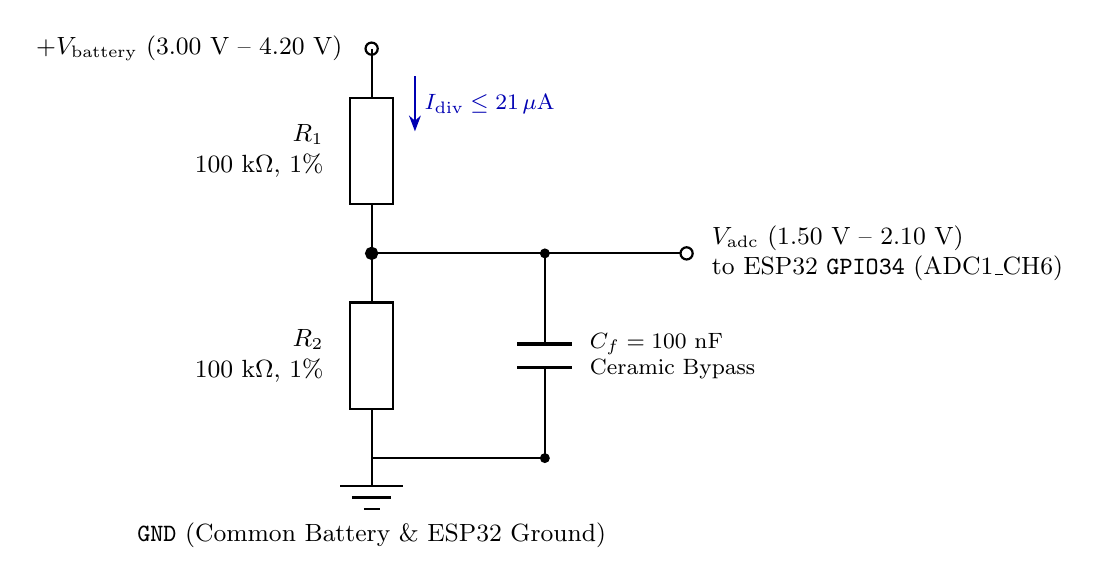
\begin{tikzpicture}[
    thick,
    res/.style={rectangle, draw=black, thick, minimum width=0.55cm, minimum height=1.35cm, fill=white},
    node font=\small
]
\coordinate (top) at (0, 5.2);
\coordinate (mid) at (0, 2.6);
\coordinate (bot) at (0, 0);
\coordinate (adc_out) at (4.0, 2.6);
\coordinate (cap_top) at (2.2, 2.6);
\coordinate (cap_mid) at (2.2, 1.3);
\coordinate (cap_bot) at (2.2, 0);

\draw[fill=white] (top) circle (2.2pt);
\node[left=0.25cm of top] {$+V_{\text{battery}}$ (3.00 V -- 4.20 V)};

\draw (top) -- (0, 4.58);
\node[res] (R1) at (0, 3.9) {};
\node[left=0.2cm of R1, align=right] {$R_1$\\$100\text{ k}\Omega$, 1\%};
\draw (0, 3.22) -- (mid);

\draw[-{Stealth[length=2mm]}, blue!70!black] (0.55, 4.85) -- node[right, font=\footnotesize] {$I_{\text{div}} \le 21\,\mu\text{A}$} (0.55, 4.15);

\draw[fill=black] (mid) circle (2pt);

\draw (mid) -- (0, 1.98);
\node[res] (R2) at (0, 1.3) {};
\node[left=0.2cm of R2, align=right] {$R_2$\\$100\text{ k}\Omega$, 1\%};
\draw (0, 0.62) -- (bot);

\draw (mid) -- (adc_out);
\draw[fill=white] (adc_out) circle (2.2pt);
\node[right=0.2cm of adc_out, align=left] {$V_{\text{adc}}$ (1.50 V -- 2.10 V)\\to ESP32 \texttt{GPIO34} (ADC1\_CH6)};

\draw (cap_top) -- (2.2, 1.45);
\draw[very thick] (1.85, 1.45) -- (2.55, 1.45);
\draw[very thick] (1.85, 1.15) -- (2.55, 1.15);
\draw (2.2, 1.15) -- (cap_bot);
\fill[black] (cap_top) circle (1.8pt);
\fill[black] (cap_bot) circle (1.8pt);
\node[right=0.45cm of cap_mid, font=\footnotesize, align=left] {$C_f = 100\text{ nF}$\\Ceramic Bypass};

\draw (bot) -- (cap_bot);
\draw (0, 0) -- (0, -0.35);
\draw (-0.4, -0.35) -- (0.4, -0.35);
\draw (-0.25, -0.5) -- (0.25, -0.5);
\draw (-0.1, -0.65) -- (0.1, -0.65);
\node[below=0.7cm of bot] {\texttt{GND} (Common Battery \& ESP32 Ground)};
\end{tikzpicture}
\caption{Voltage Divider and Bypass Filter Schematic ($R_1 = R_2 = 100\text{ k}\Omega$, $C_f = 100\text{ nF}$).}
\label{fig:voltage_divider}
\end{figure}

\subsection{Complete Hardware Connection Diagram and Pin Mapping}
Figure~\ref{fig:hw_connections} shows the complete electrical wiring between the ESP32 DevKit V1 and all peripherals, and Table~\ref{tab:pin_map} summarizes the exact pin assignments coded into the firmware.

\begin{figure}[H]
\centering
\resizebox{\linewidth}{!}{%
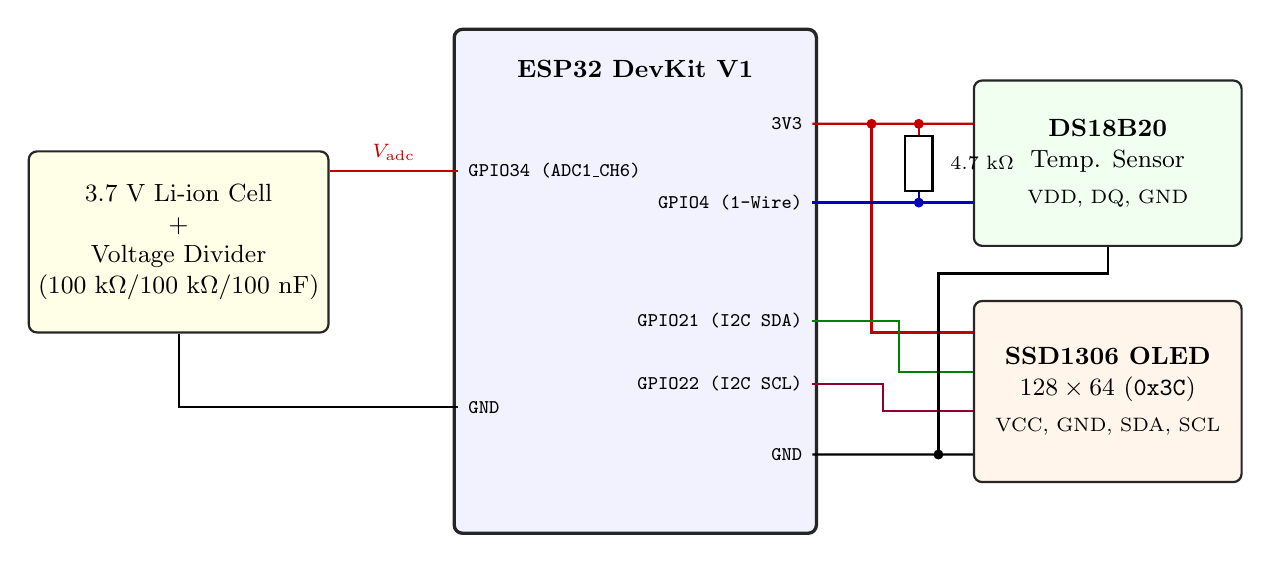
\begin{tikzpicture}[
    thick,
    ic/.style={rectangle, draw=black!85, very thick, rounded corners=3pt, fill=blue!5, align=center},
    periph/.style={rectangle, draw=black!85, thick, rounded corners=3pt, fill=green!6, align=center, font=\small},
    pinlbl/.style={font=\ttfamily\scriptsize},
    wire/.style={thick}
]

% Central ESP32 DevKit V1
\node[ic, minimum width=4.6cm, minimum height=6.4cm] (esp) at (0,0) {};
\node[font=\bfseries\small, align=center] at (0, 2.7) {ESP32 DevKit V1};

% Left-side pins
\node[pinlbl, anchor=west] (p_adc) at (-2.25, 1.4) {GPIO34 (ADC1\_CH6)};
\node[pinlbl, anchor=west] (p_gnd1) at (-2.25, -1.6) {GND};

% Right-side pins
\node[pinlbl, anchor=east] (p_3v3) at (2.25, 2.0) {3V3};
\node[pinlbl, anchor=east] (p_ow) at (2.25, 1.0) {GPIO4 (1-Wire)};
\node[pinlbl, anchor=east] (p_sda) at (2.25, -0.5) {GPIO21 (I2C SDA)};
\node[pinlbl, anchor=east] (p_scl) at (2.25, -1.3) {GPIO22 (I2C SCL)};
\node[pinlbl, anchor=east] (p_gnd2) at (2.25, -2.2) {GND};

% Left Peripheral: Battery + Voltage Divider
\node[periph, minimum width=3.6cm, minimum height=2.3cm, fill=yellow!10] (vdivbox) at (-5.8, 0.5) {3.7 V Li-ion Cell\\+\\Voltage Divider\\($100\text{ k}\Omega / 100\text{ k}\Omega / 100\text{ nF}$)};

% Right Top Peripheral: DS18B20
\node[periph, minimum width=3.4cm, minimum height=2.1cm] (ds) at (6.0, 1.5) {\textbf{DS18B20}\\Temp. Sensor\\[2pt]\scriptsize VDD, DQ, GND};
\coordinate (ds_vdd) at ($(ds.west) + (0, 0.5)$);
\coordinate (ds_dq)  at ($(ds.west) + (0, -0.5)$);

% Pull-up resistor for 1-Wire
\node[rectangle, draw=black, fill=white, minimum width=0.35cm, minimum height=0.7cm] (rpu) at (3.6, 1.5) {};
\node[right=0.08cm of rpu, font=\scriptsize] {$4.7\text{ k}\Omega$};

% Right Bottom Peripheral: SSD1306 OLED
\node[periph, minimum width=3.4cm, minimum height=2.3cm, fill=orange!8] (oled) at (6.0, -1.4) {\textbf{SSD1306 OLED}\\$128 \times 64$ (\texttt{0x3C})\\[2pt]\scriptsize VCC, GND, SDA, SCL};
\coordinate (oled_vcc) at ($(oled.west) + (0, 0.75)$);
\coordinate (oled_sda) at ($(oled.west) + (0, 0.25)$);
\coordinate (oled_scl) at ($(oled.west) + (0, -0.25)$);
\coordinate (oled_gnd) at ($(oled.west) + (0, -0.80)$);

% Left-side wiring
\draw[wire, red!75!black] (vdivbox.east |- p_adc) -- node[above, font=\scriptsize] {$V_{\text{adc}}$} (p_adc.west);
\draw[wire, black] (vdivbox.south) |- (p_gnd1.west);

% 3V3 power rail wiring
\draw[wire, red!75!black] (p_3v3.east) -- (ds_vdd);
\draw[wire, red!75!black] (3.6, 2.0) -- (rpu.north);
\draw[wire, red!75!black] (3.0, 2.0) |- (oled_vcc);

% 1-Wire DQ wiring
\draw[wire, blue!75!black] (p_ow.east) -- (ds_dq);
\draw[wire, blue!75!black] (rpu.south) -- (3.6, 1.0);
\fill[blue!75!black] (3.6, 1.0) circle (1.8pt);
\fill[red!75!black] (3.6, 2.0) circle (1.8pt);
\fill[red!75!black] (3.0, 2.0) circle (1.8pt);

% I2C SDA & SCL wiring
\draw[wire, green!50!black] (p_sda.east) -- ++(1.1,0) |- (oled_sda);
\draw[wire, purple!75!black] (p_scl.east) -- ++(0.9,0) |- (oled_scl);

% Right-side GND rail wiring
\draw[wire, black] (p_gnd2.east) -- (oled_gnd);
\draw[wire, black] (3.85, -2.2) |- (4.1, 0.1) -| (ds.south);
\fill[black] (3.85, -2.2) circle (1.8pt);
\end{tikzpicture}%
}
\caption{Complete Hardware Connection Diagram for the Proposed Battery Monitoring System.}
\label{fig:hw_connections}
\end{figure}

\begin{table}[H]
\centering
\caption{Hardware Pin Mapping Between ESP32 DevKit V1 and Peripherals}
\label{tab:pin_map}
\renewcommand{\arraystretch}{1.2}
\begin{tabular}{@{}llll@{}}
\toprule
\textbf{Peripheral / Signal} & \textbf{Peripheral Pin} & \textbf{ESP32 DevKit V1 Pin} & \textbf{Configuration / Notes} \\
\midrule
Voltage Divider Output & $V_{\text{adc}}$ & \texttt{GPIO34} & ADC1\_CH6, 12-bit, 12~dB atten. \\
Li-ion Battery Negative & $-$ Terminal & \texttt{GND} & Shared ground reference \\
DS18B20 Power & VDD & \texttt{3V3} & Dedicated 3.3~V supply \\
DS18B20 Data & DQ & \texttt{GPIO4} & Open-drain + $4.7\text{ k}\Omega$ pull-up \\
DS18B20 Ground & GND & \texttt{GND} & Shared ground \\
SSD1306 Power & VCC / GND & \texttt{3V3} / \texttt{GND} & 3.3~V logic level \\
SSD1306 I2C Data & SDA & \texttt{GPIO21} & I2C0 Master, 400~kHz \\
SSD1306 I2C Clock & SCL & \texttt{GPIO22} & I2C0 Master, 400~kHz \\
\bottomrule
\end{tabular}
\end{table}

% ----------------------------------------------------------------------------
% 11. WORKING PRINCIPLE
% ----------------------------------------------------------------------------
\section{Working Principle}
\label{sec:working_principle}

Operation of the proposed Battery Monitoring System proceeds in a deterministic 2-second periodic supervision cycle:

\begin{enumerate}
    \item \textbf{System Boot and Initialization:} When powered via USB, the ESP32 boots FreeRTOS and starts \texttt{app\_main()}. The firmware configures ADC1\_CH6 (GPIO34) at 12-bit resolution and 12~dB attenuation, creates an eFuse line-fitting calibration handle, sets GPIO4 to open-drain mode for 1-Wire communication, initializes the I2C0 master controller on GPIO21/GPIO22 at 400~kHz, and transmits the SSD1306 initialization sequence to clear and activate the OLED display.
    \item \textbf{Voltage Sensing and Noise Reduction:} The cell voltage passes continuously through the $100\text{ k}\Omega / 100\text{ k}\Omega$ divider ($0.5\times$) and $100\text{ nF}$ filter. The firmware takes 64 consecutive ADC readings, converts each via calibration to millivolts, computes the arithmetic mean $\bar{V}_{\text{adc}}$, and multiplies by $(R_1 + R_2)/R_2 = 2.0$ to reconstruct $V_{\text{battery}}$.
    \item \textbf{SOC Computation:} Reconstructed $V_{\text{battery}}$ is looked up in an 11-point ascending OCV--SOC table. If $V_{\text{battery}}$ lies between adjacent entries, piecewise linear interpolation computes the fractional percentage; values outside $[3.00\text{ V}, 4.20\text{ V}]$ saturate at 0\% or 100\%.
    \item \textbf{Digital Temperature Reading:} The ESP32 issues a 1-Wire reset pulse, sends \texttt{Skip ROM (0xCC)} and \texttt{Convert T (0x44)}, yields the CPU for 750~ms via \texttt{vTaskDelay()} while the DS18B20 digitizes temperature, reads the 9-byte scratchpad, verifies the 8-bit CRC, and scales the signed 16-bit result by $1/16\,^\circ\text{C}$.
    \item \textbf{Warning Evaluation and Display Refresh:} Hysteresis thresholds evaluate low-battery and high-temperature warning states. All metrics and alert statuses are rendered into a 1024-byte OLED framebuffer and flushed over I2C, while simultaneously logged over UART for debugging.
\end{enumerate}

% ----------------------------------------------------------------------------
% 12. SOFTWARE ARCHITECTURE
% ----------------------------------------------------------------------------
\section{Software Architecture}
\label{sec:software_architecture}

The proposed C firmware is organized into four clean functional layers (Figure~\ref{fig:sw_architecture}) implemented inside a single cohesive ESP-IDF application file (\texttt{main/main.c}) so that hardware abstractions remain clearly separated from battery algorithms.

\begin{figure}[H]
\centering
\resizebox{\linewidth}{!}{%
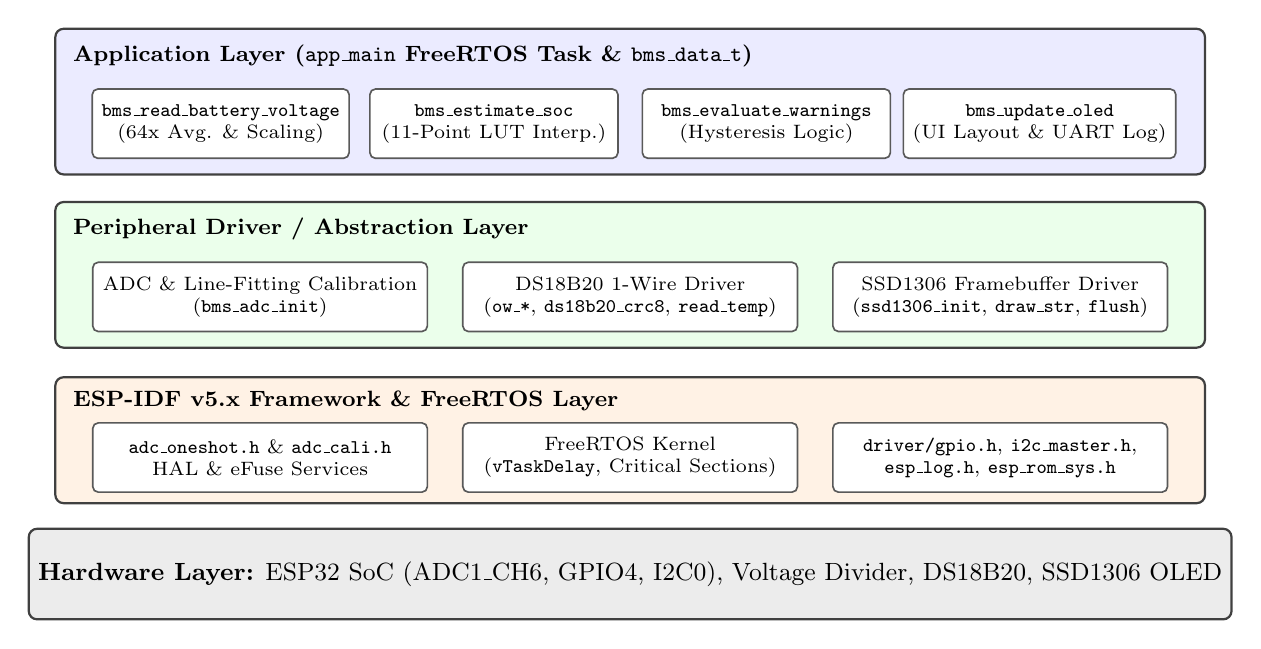
\begin{tikzpicture}[
    layer/.style={rectangle, draw=black!75, thick, rounded corners=3pt, align=center, font=\small},
    mod/.style={rectangle, draw=black!65, semithick, rounded corners=2pt, minimum height=0.88cm, minimum width=3.15cm, align=center, font=\scriptsize, fill=white}
]

\node[layer, fill=blue!8, minimum width=14.6cm, minimum height=1.85cm] (L4) at (0, 6.0) {};
\node[font=\footnotesize\bfseries, anchor=north west] at (-7.2, 6.85) {Application Layer (\texttt{app\_main} FreeRTOS Task \& \texttt{bms\_data\_t})};
\node[mod] at (-5.2, 5.72) {\texttt{bms\_read\_battery\_voltage}\\(64x Avg. \& Scaling)};
\node[mod] at (-1.73, 5.72) {\texttt{bms\_estimate\_soc}\\(11-Point LUT Interp.)};
\node[mod] at (1.73, 5.72) {\texttt{bms\_evaluate\_warnings}\\(Hysteresis Logic)};
\node[mod] at (5.2, 5.72) {\texttt{bms\_update\_oled}\\(UI Layout \& UART Log)};

\node[layer, fill=green!8, minimum width=14.6cm, minimum height=1.85cm] (L3) at (0, 3.8) {};
\node[font=\footnotesize\bfseries, anchor=north west] at (-7.2, 4.65) {Peripheral Driver / Abstraction Layer};
\node[mod, minimum width=4.25cm] at (-4.7, 3.52) {ADC \& Line-Fitting Calibration\\(\texttt{bms\_adc\_init})};
\node[mod, minimum width=4.25cm] at (0, 3.52) {DS18B20 1-Wire Driver\\(\texttt{ow\_*}, \texttt{ds18b20\_crc8}, \texttt{read\_temp})};
\node[mod, minimum width=4.25cm] at (4.7, 3.52) {SSD1306 Framebuffer Driver\\(\texttt{ssd1306\_init}, \texttt{draw\_str}, \texttt{flush})};

\node[layer, fill=orange!10, minimum width=14.6cm, minimum height=1.6cm] (L2) at (0, 1.7) {};
\node[font=\footnotesize\bfseries, anchor=north west] at (-7.2, 2.45) {ESP-IDF v5.x Framework \& FreeRTOS Layer};
\node[mod, minimum width=4.25cm] at (-4.7, 1.48) {\texttt{adc\_oneshot.h} \& \texttt{adc\_cali.h}\\HAL \& eFuse Services};
\node[mod, minimum width=4.25cm] at (0, 1.48) {FreeRTOS Kernel\\(\texttt{vTaskDelay}, Critical Sections)};
\node[mod, minimum width=4.25cm] at (4.7, 1.48) {\texttt{driver/gpio.h}, \texttt{i2c\_master.h},\\\texttt{esp\_log.h}, \texttt{esp\_rom\_sys.h}};

\node[layer, fill=gray!15, minimum width=14.6cm, minimum height=1.15cm] (L1) at (0, 0.0) {\textbf{Hardware Layer:} ESP32 SoC (ADC1\_CH6, GPIO4, I2C0), Voltage Divider, DS18B20, SSD1306 OLED};

\end{tikzpicture}%
}
\caption{Layered Software Module Architecture of the Proposed ESP-IDF C Firmware.}
\label{fig:sw_architecture}
\end{figure}

% ----------------------------------------------------------------------------
% 13. ALGORITHM AND FLOWCHART
% ----------------------------------------------------------------------------
\section{Algorithm and Flowchart}
\label{sec:algorithm_flowchart}

Figure~\ref{fig:firmware_flowchart} depicts the complete control flow executed inside \texttt{app\_main()}.

\begin{figure}[H]
\centering
\resizebox{0.80\linewidth}{!}{%
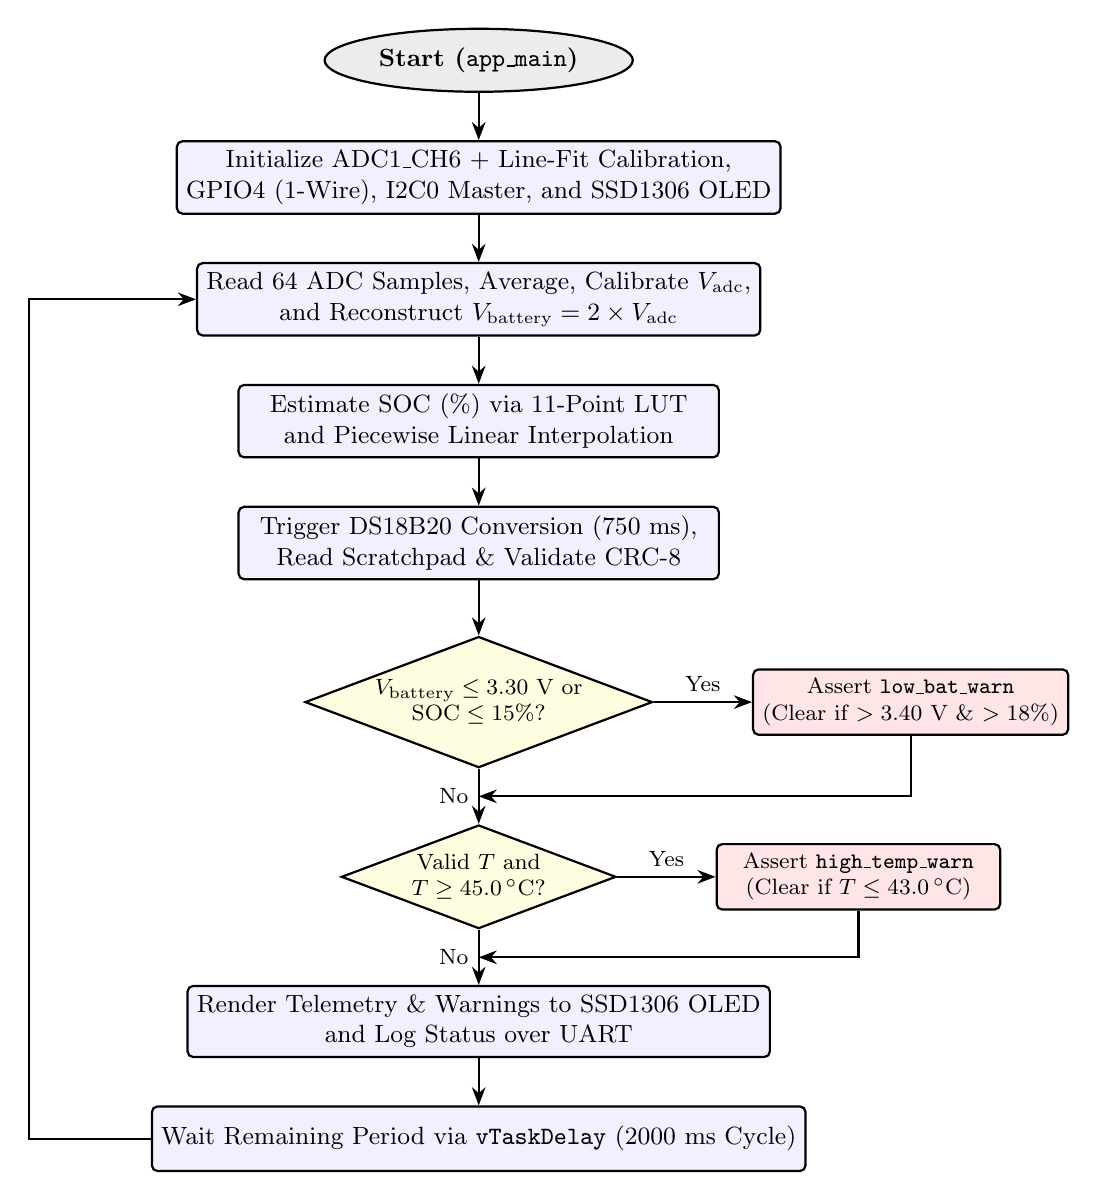
\begin{tikzpicture}[
    node distance=0.6cm,
    startstop/.style={ellipse, draw=black, thick, fill=gray!15, minimum width=3.0cm, minimum height=0.8cm, align=center, font=\small\bfseries},
    process/.style={rectangle, draw=black, thick, rounded corners=2pt, fill=blue!6, minimum width=6.1cm, minimum height=0.82cm, align=center, font=\small},
    decision/.style={diamond, draw=black, thick, fill=yellow!12, aspect=2.65, inner sep=1pt, align=center, font=\footnotesize},
    sideproc/.style={rectangle, draw=black, thick, rounded corners=2pt, fill=red!10, minimum width=3.6cm, minimum height=0.72cm, align=center, font=\footnotesize},
    arr/.style={-{Stealth[length=2.3mm]}, thick}
]

\node[startstop] (start) {Start (\texttt{app\_main})};
\node[process, below=of start] (init) {Initialize ADC1\_CH6 + Line-Fit Calibration,\\GPIO4 (1-Wire), I2C0 Master, and SSD1306 OLED};
\node[process, below=of init] (sample) {Read 64 ADC Samples, Average, Calibrate $V_{\text{adc}}$,\\and Reconstruct $V_{\text{battery}} = 2 \times V_{\text{adc}}$};
\node[process, below=of sample] (soc) {Estimate SOC (\%) via 11-Point LUT\\and Piecewise Linear Interpolation};
\node[process, below=of soc] (temp) {Trigger DS18B20 Conversion (750 ms),\\Read Scratchpad \& Validate CRC-8};
\node[decision, below=0.7cm of temp] (lowbat) {$V_{\text{battery}} \le 3.30\text{ V}$ or\\$\text{SOC} \le 15\%$?};
\node[sideproc, right=1.25cm of lowbat] (setlow) {Assert \texttt{low\_bat\_warn}\\(Clear if $>3.40\text{ V}$ \& $>18\%$)};
\node[decision, below=0.7cm of lowbat] (hightemp) {Valid $T$ and\\$T \ge 45.0\,^\circ\text{C}$?};
\node[sideproc, right=1.25cm of hightemp] (sethigh) {Assert \texttt{high\_temp\_warn}\\(Clear if $T \le 43.0\,^\circ\text{C}$)};
\node[process, below=0.7cm of hightemp] (disp) {Render Telemetry \& Warnings to SSD1306 OLED\\and Log Status over UART};
\node[process, below=of disp] (delay) {Wait Remaining Period via \texttt{vTaskDelay} (2000 ms Cycle)};

\draw[arr] (start) -- (init);
\draw[arr] (init) -- (sample);
\draw[arr] (sample) -- (soc);
\draw[arr] (soc) -- (temp);
\draw[arr] (temp) -- (lowbat);
\draw[arr] (lowbat) -- node[left, font=\footnotesize] {No} (hightemp);
\draw[arr] (lowbat) -- node[above, font=\footnotesize] {Yes} (setlow);
\draw[arr] (setlow.south) |- ($(lowbat.south)!0.5!(hightemp.north)$);
\draw[arr] (hightemp) -- node[left, font=\footnotesize] {No} (disp);
\draw[arr] (hightemp) -- node[above, font=\footnotesize] {Yes} (sethigh);
\draw[arr] (sethigh.south) |- ($(hightemp.south)!0.5!(disp.north)$);
\draw[arr] (disp) -- (delay);

\draw[arr] (delay.west) -- ++(-1.55,0) |- (sample.west);
\end{tikzpicture}%
}
\caption{Firmware Execution Flowchart Implemented in \texttt{app\_main()}.}
\label{fig:firmware_flowchart}
\end{figure}

% ----------------------------------------------------------------------------
% 14. MATHEMATICAL FORMULATION
% ----------------------------------------------------------------------------
\section{Mathematical Formulation}
\label{sec:math_formulation}

\subsection{Voltage Divider Scaling and Reconstruction}
Assuming negligible steady-state ADC input leakage current, the voltage divider scales battery terminal voltage according to:
\begin{equation}
    V_{\text{adc}} = V_{\text{battery}} \times \frac{R_2}{R_1 + R_2}
    \label{eq:vdiv}
\end{equation}
Inverting~\eqref{eq:vdiv} gives the firmware reconstruction formula:
\begin{equation}
    V_{\text{battery}} = V_{\text{adc}} \times \frac{R_1 + R_2}{R_2}
    \label{eq:vbat}
\end{equation}
With $R_1 = R_2 = 100\text{ k}\Omega$, the scaling ratio is exactly $(R_1 + R_2)/R_2 = 2.0$. The continuous divider drain current and DC Thevenin source impedance are:
\begin{equation}
    I_{\text{div}} = \frac{V_{\text{battery}}}{R_1 + R_2}, \qquad R_{\text{th}} = \frac{R_1 R_2}{R_1 + R_2}
    \label{eq:idiv_rth}
\end{equation}
yielding $I_{\text{div}} = 21.0\,\mu\text{A}$ at $4.20\text{ V}$ and $R_{\text{th}} = 50\text{ k}\Omega$. If $R_1$ and $R_2$ have fractional manufacturing tolerances $\pm \delta_1$ and $\pm \delta_2$, first-order worst-case sensitivity yields a relative reconstruction error bound:
\begin{equation}
    \left|\frac{\Delta V_{\text{battery}}}{V_{\text{battery}}}\right|_{\max} \approx \frac{R_1}{R_1 + R_2}(\delta_1 + \delta_2)
    \label{eq:tol_err}
\end{equation}
For 1\% resistors ($\delta_1 = \delta_2 = 0.01$) with $R_1 = R_2$, the worst-case divider tolerance error is $\pm 1.0\%$ ($\pm 42\text{ mV}$ at $4.20\text{ V}$), which can be further reduced in hardware by measuring actual resistor values with a multimeter and updating \texttt{VDIV\_R1\_OHM} and \texttt{VDIV\_R2\_OHM}.

\subsection{ADC Quantization and Multi-Sample Averaging}
For a 12-bit ADC across an effective full-scale span $V_{\text{FS}}$, the ideal quantization step is:
\begin{equation}
    \Delta V_{\text{LSB}} = \frac{V_{\text{FS}}}{2^{12} - 1} = \frac{V_{\text{FS}}}{4095}
    \label{eq:adc_lsb}
\end{equation}
At $V_{\text{FS}} \approx 3.10\text{ V}$ (12~dB attenuation), $\Delta V_{\text{LSB}} \approx 0.76\text{ mV}$ at the ADC pin, corresponding to $\approx 1.51\text{ mV}$ referred to the battery terminals. Averaging $N = 64$ calibrated readings:
\begin{equation}
    \bar{V}_{\text{adc}} = \frac{1}{N} \sum_{k=1}^{N} V_{\text{adc},k}
    \label{eq:adc_avg}
\end{equation}
reduces the standard deviation of uncorrelated zero-mean noise by a factor of $\sqrt{N} = 8$.

\subsection{Piecewise Linear SOC Interpolation and Load Model}
Given adjacent lookup points $(V_1, \text{SOC}_1)$ and $(V_2, \text{SOC}_2)$ bracketing reconstructed voltage $V$ ($V_1 \le V \le V_2$), linear interpolation yields:
\begin{equation}
    \text{SOC} = \text{SOC}_1 + \left(\frac{V - V_1}{V_2 - V_1}\right) \times (\text{SOC}_2 - \text{SOC}_1)
    \label{eq:soc_interp}
\end{equation}
Under load current $I_{\text{load}}$, terminal voltage departs from Open-Circuit Voltage according to the first-order equivalent-circuit model~\cite{plett_bms1}:
\begin{equation}
    V_{\text{term}} = V_{\text{OCV}}(\text{SOC}, T) - I_{\text{load}} \cdot R_{\text{int}}(\text{SOC}, T, \text{SOH})
    \label{eq:vterm}
\end{equation}

% ----------------------------------------------------------------------------
% 15. C FIRMWARE IMPLEMENTATION
% ----------------------------------------------------------------------------
\section{C Firmware Implementation}
\label{sec:firmware_impl}

The complete proposed C firmware (\texttt{main/main.c}) is provided in Appendix~\ref{app:source_code}. Every software component documented below maps directly to the code in Listing~\ref{lst:main_c}.

\subsection{Header Files, Configuration Macros, and Data Structures}
The firmware imports standard C headers (\texttt{<stdio.h>}, \texttt{<stdint.h>}, \texttt{<stdbool.h>}, \texttt{<string.h>}), FreeRTOS task headers (\texttt{freertos/FreeRTOS.h}, \texttt{freertos/task.h}), ESP-IDF logging/timing utilities (\texttt{esp\_log.h}, \texttt{esp\_err.h}, \texttt{esp\_rom\_sys.h}), and modern ESP-IDF v5.x peripheral drivers (\texttt{driver/gpio.h}, \texttt{driver/i2c\_master.h}, \texttt{esp\_adc/adc\_oneshot.h}, \texttt{esp\_adc/adc\_cali.h}, \texttt{esp\_adc/adc\_cali\_scheme.h}). Hardware constants (\texttt{BAT\_ADC\_CHANNEL}, \texttt{VDIV\_R1\_OHM}, \texttt{VDIV\_R2\_OHM}, \texttt{DS18B20\_GPIO}, \texttt{I2C\_SDA\_GPIO}, \texttt{I2C\_SCL\_GPIO}, \texttt{SSD1306\_I2C\_ADDR}) and alert thresholds are centralized via preprocessor macros for clean configurability. Two C structures organize runtime data:
\begin{itemize}
    \item \texttt{soc\_point\_t}: Pairs a resting cell voltage (\texttt{voltage\_v}) with its reference percentage (\texttt{soc\_pct}) inside the read-only \texttt{const} lookup array \texttt{soc\_lut[]}.
    \item \texttt{bms\_data\_t}: Aggregates all instantaneous measurements (\texttt{adc\_voltage\_v}, \texttt{battery\_voltage\_v}, \texttt{soc\_pct}, \texttt{temp\_c}, \texttt{temp\_valid}) and latched warning flags (\texttt{low\_bat\_warn}, \texttt{high\_temp\_warn}).
\end{itemize}

\subsection{ADC Initialization and eFuse Calibration}
The function \texttt{bms\_adc\_init()} instantiates ADC1 via \texttt{adc\_oneshot\_new\_unit()} and configures \texttt{ADC\_CHANNEL\_6} (GPIO34) with \texttt{ADC\_ATTEN\_DB\_12} and \texttt{ADC\_BITWIDTH\_12}. It then attempts to initialize ESP32 factory line-fitting calibration via \texttt{adc\_cali\_create\_scheme\_line\_fitting()}. If calibration succeeds, \texttt{s\_adc\_calibrated} is set to \texttt{true}; if eFuse data are unavailable on a particular chip, the firmware logs a warning and automatically falls back to nominal 3.10~V linear scaling rather than crashing.

\subsection{Voltage Sampling, Averaging, and Reconstruction}
The function \texttt{bms\_read\_battery\_voltage()} executes a 64-iteration loop calling \texttt{adc\_oneshot\_read()}. When calibrated, each sample is immediately converted to millivolts using \texttt{adc\_cali\_raw\_to\_voltage()} and accumulated in a 64-bit integer sum to prevent overflow. The average ADC voltage in volts is stored in \texttt{data->adc\_voltage\_v}, and battery terminal voltage is reconstructed via \texttt{data->adc\_voltage\_v * ((VDIV\_R1\_OHM + VDIV\_R2\_OHM) / VDIV\_R2\_OHM)}, directly realizing~\eqref{eq:vbat}.

\subsection{Charge Percentage Lookup and Interpolation}
The function \texttt{bms\_estimate\_soc(float v\_bat)} handles boundary clamping first (returning \texttt{0.0f} if $V \le 3.00\text{ V}$ and \texttt{100.0f} if $V \ge 4.20\text{ V}$). Otherwise, it iterates through \texttt{soc\_lut[]} to locate the interval $[V_i, V_{i+1}]$ containing \texttt{v\_bat} and evaluates~\eqref{eq:soc_interp} in single-precision floating point.

\subsection{DS18B20 1-Wire Acquisition and SSD1306 I2C Rendering}
Low-level 1-Wire signaling (\texttt{ow\_reset}, \texttt{ow\_write\_bit}, \texttt{ow\_read\_bit}) uses open-drain control on GPIO4 with \texttt{esp\_rom\_delay\_us()} enclosed in FreeRTOS spinlock critical sections (\texttt{portENTER\_CRITICAL}) so preemption never corrupts microsecond timing slots. \texttt{ds18b20\_read\_temp()} triggers conversion, yields 750~ms via \texttt{vTaskDelay()}, reads all 9 scratchpad bytes, checks \texttt{ds18b20\_crc8()}, and returns \texttt{ESP\_OK} only when both sensor presence and CRC pass. On the display side, \texttt{ssd1306\_init()} registers device \texttt{0x3C} on the ESP-IDF v5.x I2C master bus and initializes the OLED controller; \texttt{bms\_update\_oled()} draws formatted strings using a compact built-in $5 \times 7$ bitmap font into \texttt{s\_oled\_fb[1024]} and flushes all 8 pages via \texttt{ssd1306\_flush()}.

\subsection{Main Loop and Error Handling}
In \texttt{app\_main()}, critical hardware initialization calls (ADC and I2C/OLED) are checked with \texttt{ESP\_ERROR\_CHECK()}. Inside the infinite monitoring loop, transient ADC or DS18B20 faults are handled non-fatally: if \texttt{ds18b20\_read\_temp()} fails (e.g., loose sensor wire or CRC mismatch), \texttt{temp\_valid} is set to \texttt{false}, the OLED displays \texttt{T:ERR}, and the system continues monitoring battery voltage safely. Periodic loop execution is governed by FreeRTOS \texttt{vTaskDelayUntil()} configured for a strict, deterministic $2000\text{ ms}$ sampling cadence regardless of sensor response times or bus latency.

% ----------------------------------------------------------------------------
% 16. BATTERY PERCENTAGE ESTIMATION METHOD
% ----------------------------------------------------------------------------
\section{Battery Percentage Estimation Method}
\label{sec:soc_estimation}

Table~\ref{tab:soc_lut} lists the exact 11-point resting OCV--SOC lookup table embedded in \texttt{soc\_lut[]} in Appendix~\ref{app:source_code}, representative of a standard 3.7~V Li-ion cell at $25\,^\circ\text{C}$~\cite{reddy_linden}.

\begin{table}[H]
\centering


\renewcommand{\arraystretch}{1.15}
\begin{tabular}{|@{}c|c|c|c@{}|}
\hline
\textbf{Voltage $V$ (V)} & \textbf{SOC (\%)} & \textbf{Voltage $V$ (V)} & \textbf{SOC (\%)} \\
\hline
3.00 & 0.0  & 3.84 & 60.0 \\\hline
3.50 & 10.0 & 3.93 & 70.0 \\\hline
3.61 & 20.0 & 4.02 & 80.0 \\\hline
3.66 & 30.0 & 4.11 & 90.0 \\\hline
3.70 & 40.0 & 4.20 & 100.0 \\\hline
3.74 & 50.0 & ---  & ---  \\
\hline
\end{tabular}
\caption{11-Point Resting OCV--SOC Lookup Table Embedded in Firmware (\texttt{soc\_lut[]})}
\label{tab:soc_lut}
\end{table}

\subsection{Worked Interpolation Examples}
Applying~\eqref{eq:soc_interp} to two intermediate voltages:
\begin{itemize}
    \item At $V = 3.78\text{ V}$ (between $3.74\text{ V}$ at 50\% and $3.84\text{ V}$ at 60\%):
    \[\text{SOC} = 50 + \frac{3.78 - 3.74}{3.84 - 3.74} \times (60 - 50) = 54.0\%\]
    \item At $V = 3.30\text{ V}$ (between $3.00\text{ V}$ at 0\% and $3.50\text{ V}$ at 10\%):
    \[\text{SOC} = 0 + \frac{3.30 - 3.00}{3.50 - 3.00} \times (10 - 0) = 6.0\%\]
\end{itemize}

\subsection{Limitations of Voltage-Based SOC Estimation}
Voltage-only SOC estimation carries four inherent electrochemical limitations~\cite{plett_bms1, plett_bms2}:
\begin{enumerate}
    \item \textbf{Load Current Effects (IR Drop):} As modeled in~\eqref{eq:vterm}, discharge current causes a terminal voltage drop $I_{\text{load}} \cdot R_{\text{int}}$, making estimated SOC read artificially low while under load and rebound after load removal. Conversely, charging elevates terminal voltage above $V_{\text{OCV}}$, causing overestimation.
    \item \textbf{Mid-Plateau Sensitivity:} Between 3.66~V (30\%) and 3.74~V (50\%), a slope of $250\%/\text{V}$ means even a $20\text{ mV}$ ADC or resistor-tolerance error introduces a 5\% SOC error.
    \item \textbf{Temperature Effects:} Low temperatures increase electrolyte resistance and reduce usable capacity, depressing terminal voltage for the same true SOC.
    \item \textbf{Chemistry and Aging Variation:} Different chemistries (e.g., LFP vs.\ NMC/LCO) have different OCV curves, and aged cells exhibit higher $R_{\text{int}}$ and shifted discharge knees.
\end{enumerate}

% ----------------------------------------------------------------------------
% 17. TEMPERATURE MONITORING
% ----------------------------------------------------------------------------
\section{Temperature Monitoring}
\label{sec:temp_monitoring}

Standard Li-ion cells specify safe charging between $0\,^\circ\text{C}$ and $45\,^\circ\text{C}$ and safe discharging up to $60\,^\circ\text{C}$~\cite{reddy_linden}. Mounting the DS18B20 in firm thermal contact with the Li-ion cell casing enables accurate tracking of thermal rise. In the proposed firmware, \texttt{ds18b20\_read\_temp()} enforces strict 1-Wire protocol timing using critical sections around each bit slot, waits the full datasheet-specified 750~ms conversion time at 12-bit resolution ($0.0625\,^\circ\text{C}$/LSB) without blocking other FreeRTOS tasks, and validates all received scratchpad bytes using the Maxim polynomial $x^8 + x^5 + x^4 + 1$ (reflected byte \texttt{0x8C}). Any missing presence pulse or CRC failure immediately flags \texttt{temp\_valid = false} so corrupted readings (such as the power-on default $85.0\,^\circ\text{C}$ or disconnected $-127\,^\circ\text{C}$) never trigger false alarms.

% ----------------------------------------------------------------------------
% 18. WARNING AND ALERT MECHANISM
% ----------------------------------------------------------------------------
\section{Warning and Alert Mechanism}
\label{sec:warnings}

The function \texttt{bms\_evaluate\_warnings()} implements dual threshold monitoring with built-in hysteresis to prevent display chatter when measurements hover near a limit:
\begin{itemize}
    \item \textbf{Low-Battery Warning:} Asserts \texttt{low\_bat\_warn = true} when $V_{\text{battery}} \le 3.30\text{ V}$ or $\text{SOC} \le 15.0\%$. It clears only when $V_{\text{battery}} \ge 3.40\text{ V}$ and $\text{SOC} \ge 18.0\%$.
    \item \textbf{High-Temperature Warning:} When \texttt{temp\_valid} is true, asserts \texttt{high\_temp\_warn = true} at $T \ge 45.0\,^\circ\text{C}$ and clears only when $T \le 43.0\,^\circ\text{C}$.
\end{itemize}
Active alerts are displayed prominently on Row~6 of the SSD1306 OLED (\texttt{WARN:LOW BAT}, \texttt{WARN:HI TEMP}, or \texttt{WARN:LOW+TMP}; otherwise \texttt{STATUS: OK}) and logged as warning-level messages via \texttt{ESP\_LOGW()} over UART.

% ----------------------------------------------------------------------------
% 19. TESTING AND EXPERIMENTAL RESULTS
% ----------------------------------------------------------------------------
\section{Testing Plan, Theoretical Calculations, and Expected Results}
\label{sec:testing_results}

\textit{Transparency Statement:} Because this document is submitted as an academic project idea and complete engineering design proposal prior to physical hardware fabrication, no benchtop experimental measurements have been performed yet. Accordingly, this section presents exact \textbf{theoretical design calculations}, \textbf{expected firmware outputs}, and a \textbf{structured hardware verification protocol} for the upcoming build phase.

\subsection{Theoretical Calculations and Expected Firmware Output}
Table~\ref{tab:theoretical_calc} summarizes the theoretically expected ADC node voltage, divider drain current, interpolated SOC percentage, and warning flags across the Li-ion operating envelope for $R_1 = R_2 = 100\text{ k}\Omega$ and ambient temperature $T = 28.0\,^\circ\text{C}$.

\begin{table}[H]
\centering


\renewcommand{\arraystretch}{1.2}
\begin{tabular}{|@{}c|c|c|c|c@{}|}
\hline
\textbf{$V_{\text{battery}}$ (V)} & \textbf{Expected $V_{\text{adc}}$ (V)} & \textbf{$I_{\text{div}}$ ($\mu$A)} & \textbf{Expected SOC (\%)} & \textbf{Expected OLED Status} \\
\hline
4.20 & 2.100 & 21.0 & 100.0 & \texttt{STATUS: OK} \\\hline
3.93 & 1.965 & 19.7 & 70.0  & \texttt{STATUS: OK} \\\hline
3.78 & 1.890 & 18.9 & 54.0  & \texttt{STATUS: OK} \\\hline
3.61 & 1.805 & 18.1 & 20.0  & \texttt{STATUS: OK} \\\hline
3.55 & 1.775 & 17.8 & 14.5  & \texttt{WARN:LOW BAT} \\\hline
3.30 & 1.650 & 16.5 & 6.0   & \texttt{WARN:LOW BAT} \\\hline
3.00 & 1.500 & 15.0 & 0.0   & \texttt{WARN:LOW BAT} \\
\hline
\end{tabular}
\caption{Theoretical Calculations and Expected Firmware Output ($R_1 = R_2 = 100\text{ k}\Omega$, $T = 28.0\,^\circ\text{C}$)}
\label{tab:theoretical_calc}
\end{table}

\subsection{Planned Hardware Verification Protocol}
Upon assembling the prototype on a breadboard or PCB, the following laboratory tests will be executed and recorded in Table~\ref{tab:validation_plan}:
\begin{enumerate}
    \item \textbf{Simulated Battery Voltage Sweep:} Connect a variable benchtop DC power supply in place of the battery and sweep from 3.00~V to 4.20~V in 0.10~V steps. Compare ESP32 reconstructed voltage against a calibrated 4.5-digit digital multimeter (DMM); target error is within $\pm 30\text{ mV}$ after measuring exact $R_1, R_2$ values.
    \item \textbf{Thermal Accuracy and High-Temperature Alert Test:} Compare DS18B20 output against a reference thermometer at ambient temperature, then gently warm the sensor above $45.0\,^\circ\text{C}$ to verify alert assertion and confirm hysteresis release at $\le 43.0\,^\circ\text{C}$.
    \item \textbf{Fault Robustness Test:} Temporarily disconnect the DS18B20 DQ line to confirm \texttt{T:ERR} fault handling without crashing the OLED or voltage monitoring task.
\end{enumerate}

\begin{table}[H]
\centering


\renewcommand{\arraystretch}{1.2}
\begin{tabular}{|@{}p{3.8cm}|p{3.4cm}|p{4.0cm}|p{2.8cm}@{}|}
\hline
\textbf{Verification Test} & \textbf{Test Stimulus} & \textbf{Acceptance Criterion} & \textbf{Status} \\
\hline
Voltage Accuracy Sweep & Bench PSU 3.00--4.20~V & $|V_{\text{ESP32}} - V_{\text{DMM}}| \le 30\text{ mV}$ & Planned \\\hline
SOC Interpolation Check & Mid-interval voltages & Matches~\eqref{eq:soc_interp} within $\pm 0.5\%$ & Planned \\\hline
Low-Battery Hysteresis & Sweep 3.60~V $\to$ 3.25~V $\to$ 3.45~V & Triggers $\le 3.30\text{ V}$/15\%, clears $\ge 3.40\text{ V}$/18\% & Planned \\\hline
High-Temp.\ Hysteresis & Warm probe $> 45\,^\circ\text{C}$, cool $< 43\,^\circ\text{C}$ & Asserts at $45\,^\circ\text{C}$, clears at $43\,^\circ\text{C}$ & Planned \\\hline
1-Wire Disconnect Fault & Open DQ line & Displays \texttt{T:ERR}, voltage loop continues & Planned \\
\hline
\end{tabular}
\caption{Planned Experimental Validation Matrix (To Be Populated During Prototype Testing)}
\label{tab:validation_plan}
\end{table}

% ----------------------------------------------------------------------------
% 20. LIMITATIONS
% ----------------------------------------------------------------------------
\section{Limitations}
\label{sec:limitations}

\begin{enumerate}
    \item \textbf{Passive Monitoring Only:} The design alerts the user but does not incorporate MOSFET cutoff switches to automatically disconnect the battery during severe under-voltage or over-temperature faults.
    \item \textbf{No Current Measurement:} Without a shunt resistor or current-sense amplifier, the system cannot compensate for $I \cdot R_{\text{int}}$ load sag or perform Coulomb counting.
    \item \textbf{Internal ADC Precision Ceiling:} The ESP32 internal 12-bit SAR ADC exhibits higher integral non-linearity than external 16-bit sigma-delta ADCs (such as the ADS1115).
    \item \textbf{Constant Divider Drain:} The $200\text{ k}\Omega$ divider continuously draws roughly $15$--$21\,\mu\text{A}$ whenever the cell remains connected.
    \item \textbf{Single-Cell Topology:} The circuit supports only one 3.7~V Li-ion cell and cannot directly monitor series-connected multi-cell packs.
\end{enumerate}

% ----------------------------------------------------------------------------
% 21. FUTURE IMPROVEMENTS
% ----------------------------------------------------------------------------
\section{Future Improvements}
\label{sec:future_improvements}

\begin{enumerate}
    \item \textbf{INA219/INA226 Integration:} Adding an I2C shunt monitor would supply high-precision voltage and current readings, enabling hybrid OCV + Coulomb counting or Extended Kalman Filter SOC estimation~\cite{plett_bms2}.
    \item \textbf{IoT Wireless Telemetry:} Using the ESP32 Wi-Fi or BLE stack, real-time battery status and safety alerts can be pushed to an MQTT dashboard or smartphone app.
    \item \textbf{Active Hardware Cutoff Protection:} Integrating a DW01A protection IC with dual MOSFETs or an ESP32-driven load switch would convert the monitor into a full protection BMS.
    \item \textbf{Switched Divider and Deep Sleep:} Placing a low-$R_{\text{DS(on)}}$ MOSFET in series with the divider combined with ESP32 deep-sleep cycles would cut standby power consumption dramatically.
    \item \textbf{Audible Buzzer and Non-Volatile Logging:} Adding a piezoelectric buzzer and SPIFFS/LittleFS flash logging would improve field alerting and discharge-curve diagnostics.
\end{enumerate}

% ----------------------------------------------------------------------------
% 22. CONCLUSION
% ----------------------------------------------------------------------------
\section{Conclusion}
\label{sec:conclusion}

In this assignment, I have presented a complete, self-contained design proposal for a \textit{Battery Monitoring System Using ESP32 and C Firmware}. The proposed architecture safely interfaces a single-cell 3.7~V Li-ion battery to the ESP32 DevKit V1 using a $100\text{ k}\Omega / 100\text{ k}\Omega$ resistive voltage divider and $100\text{ nF}$ bypass filter, applies ESP-IDF v5.x eFuse line-fitting calibration with 64-sample averaging, estimates State of Charge via an 11-point piecewise linear lookup table, monitors cell temperature through a CRC-verified DS18B20 1-Wire sensor, evaluates hysteresis-protected safety warnings, and visualizes all metrics on an SSD1306 $128 \times 64$ I2C OLED display.

By uniting circuit-level analysis, electrochemical modeling of voltage-based SOC limitations, clean modular C firmware, and a rigorous pre-build validation plan, this design establishes a solid, reproducible foundation ready for physical prototype construction and bench testing.

% ----------------------------------------------------------------------------
% 23. REFERENCES
% ----------------------------------------------------------------------------
\newpage
\bibliographystyle{ieeetr}
\bibliography{reference}

% ----------------------------------------------------------------------------
% 24. APPENDIX: COMPLETE SOURCE CODE
% ----------------------------------------------------------------------------
\newpage
\appendix
\section{Complete Proposed ESP-IDF C Firmware Source Code}
\label{app:source_code}

Listing~\ref{lst:main_c} contains the complete, self-contained ESP-IDF v5.x C firmware (\texttt{main/main.c}) designed for this project.

\lstinputlisting[caption={ESP-IDF C Firmware (\texttt{main/main.c})}, label={lst:main_c}]{main/main.c}

\end{document}